% =============================================================================
% MSc thesis defense — "Building Cooperative Robot Behavior from Basic Action Modules"
% Jan M. Straub, Heidelberg University.
% =============================================================================
\documentclass[aspectratio=169,11pt]{beamer}

\usetheme{metropolis}
\metroset{numbering=fraction, progressbar=foot, block=fill}

\usepackage[utf8]{inputenc}
\usepackage[T1]{fontenc}
\usepackage{booktabs}
\usepackage{graphicx}
\usepackage{amsmath}
\usepackage{xcolor}
\usepackage{tikz}
\usepackage{multicol}

\graphicspath{{images/}}

\definecolor{hdred}{RGB}{198,24,38}
\setbeamercolor{progress bar}{fg=hdred}
\setbeamercolor{title separator}{fg=hdred}
\setbeamercolor{alerted text}{fg=hdred}

\setbeamertemplate{bibliography item}[text]
\newcommand{\bibtinyfont}{\fontsize{5}{5.8}\selectfont}
\setbeamerfont{bibliography item}{size=\bibtinyfont}
\setbeamerfont{bibliography entry author}{size=\bibtinyfont}
\setbeamerfont{bibliography entry title}{size=\bibtinyfont}
\setbeamerfont{bibliography entry location}{size=\bibtinyfont}
\setbeamerfont{bibliography entry note}{size=\bibtinyfont}
\makeatletter
\def\bstctlcite{\@ifnextchar[{\@bstctlcite}{\@bstctlcite[@auxout]}}
\def\@bstctlcite[#1]#2{\@bsphack
	\@for\@citeb:=#2\do{%
		\edef\@citeb{\expandafter\@firstofone\@citeb}%
		\if@filesw\immediate\write\csname #1\endcsname{\string\citation{\@citeb}}\fi}%
	\@esphack}
\makeatother

% Overview agenda entry: number, section name, one-line description.
\newcommand{\agendaitem}[3]{%
	\parbox[t]{1.8em}{{\color{hdred}\large\bfseries #1}}%
	\parbox[t]{\dimexpr\linewidth-1.8em\relax}{%
		\textbf{#2}\\[0.15em]
		{\small\color{black!55} #3}}\\[0.85em]}

\title{Building Cooperative Robot Behavior\\from Basic Action Modules}
\subtitle{An LLM-driven control framework for two cooperating AR4 arms}
\author{Jan M.\ Straub\\ [0.4em]{\small Supervisor: Prof.\ Dr.\ Artur Andrzejak}}
\institute{Institute for Computer Science --- Artificial Intelligence for Programming\\Ruprecht-Karls-University of Heidelberg}
\date{\today}

\begin{document}

\bstctlcite{BSTcontrol}

% =============================================================================
% OPENING
% =============================================================================
\maketitle

% --- Overview / outline ------------------------------------------------------
\begin{frame}{Overview}
	\agendaitem{1}{The problem}{The reasoning--execution gap, and why cooperation is the hard case}
	\agendaitem{2}{Pillar 1 --- Grounding}{A 20-operation vocabulary makes a small, local VLM reliable}
	\agendaitem{3}{Pillar 2 --- Cooperation emerges}{Handoffs and parallelism composed by the model}
	\agendaitem{4}{Pillar 3 --- The boundary}{The one failing task, what the ablations really show, limitations}
	\agendaitem{5}{Conclusion}{The five contributions, the path to hardware, future work}
\end{frame}

% --- Slide 2: the answer first (pyramid apex) --------------------------------
\begin{frame}{Condensed Results}
	\begin{block}{Thesis in one sentence}
		A \alert{locally hosted vision-language model (VLM)}, grounded in a structured pool of \alert{20 basic operations}, turns natural language into reliable \alert{robot behavior}, with \alert{no fine-tuning and no hard-coded sequencing}.
	\end{block}
	\vfill
	\begin{columns}[t]
		\begin{column}{0.33\textwidth}
			\begin{exampleblock}{Solved}
				1.000 success rate on all single-robot tasks and dual-arm handovers.
			\end{exampleblock}
		\end{column}
		\begin{column}{0.33\textwidth}
			\begin{exampleblock}{Emergent}
				Cooperation is reasoned, not scripted. Negotiation lifts the default model's dual-robot success.
			\end{exampleblock}
		\end{column}
		\begin{column}{0.33\textwidth}
			\begin{alertblock}{One gap}
				Concurrent bimanual lift fails: target selection is not partner-aware, plus a simulator attachment limit.
			\end{alertblock}
		\end{column}
	\end{columns}
\end{frame}

% =============================================================================
% PROBLEM & POSITIONING
% =============================================================================
\section{The Problem}

\begin{frame}{The Reasoning--Execution Gap}
	\begin{columns}[T]
		\begin{column}{0.6\textwidth}
			\footnotesize
			\begin{itemize}
				\item Classical robots: precise, but caged. Rigid paths, no tolerance for the unexpected.
				\item VLMs bring world knowledge and reasoning, but cannot reliably turn abstract reasoning into \emph{physical} action.
				\item Models often ignore \alert{past physical state} when planning the next move.
			\end{itemize}
			\begin{block}{Why cooperation is the hard case}
				Two arms must \textbf{avoid collision}, \textbf{share a workspace}, and \textbf{synchronize timing}.
			\end{block}
		\end{column}
		\begin{column}{0.4\textwidth}
			\centering
			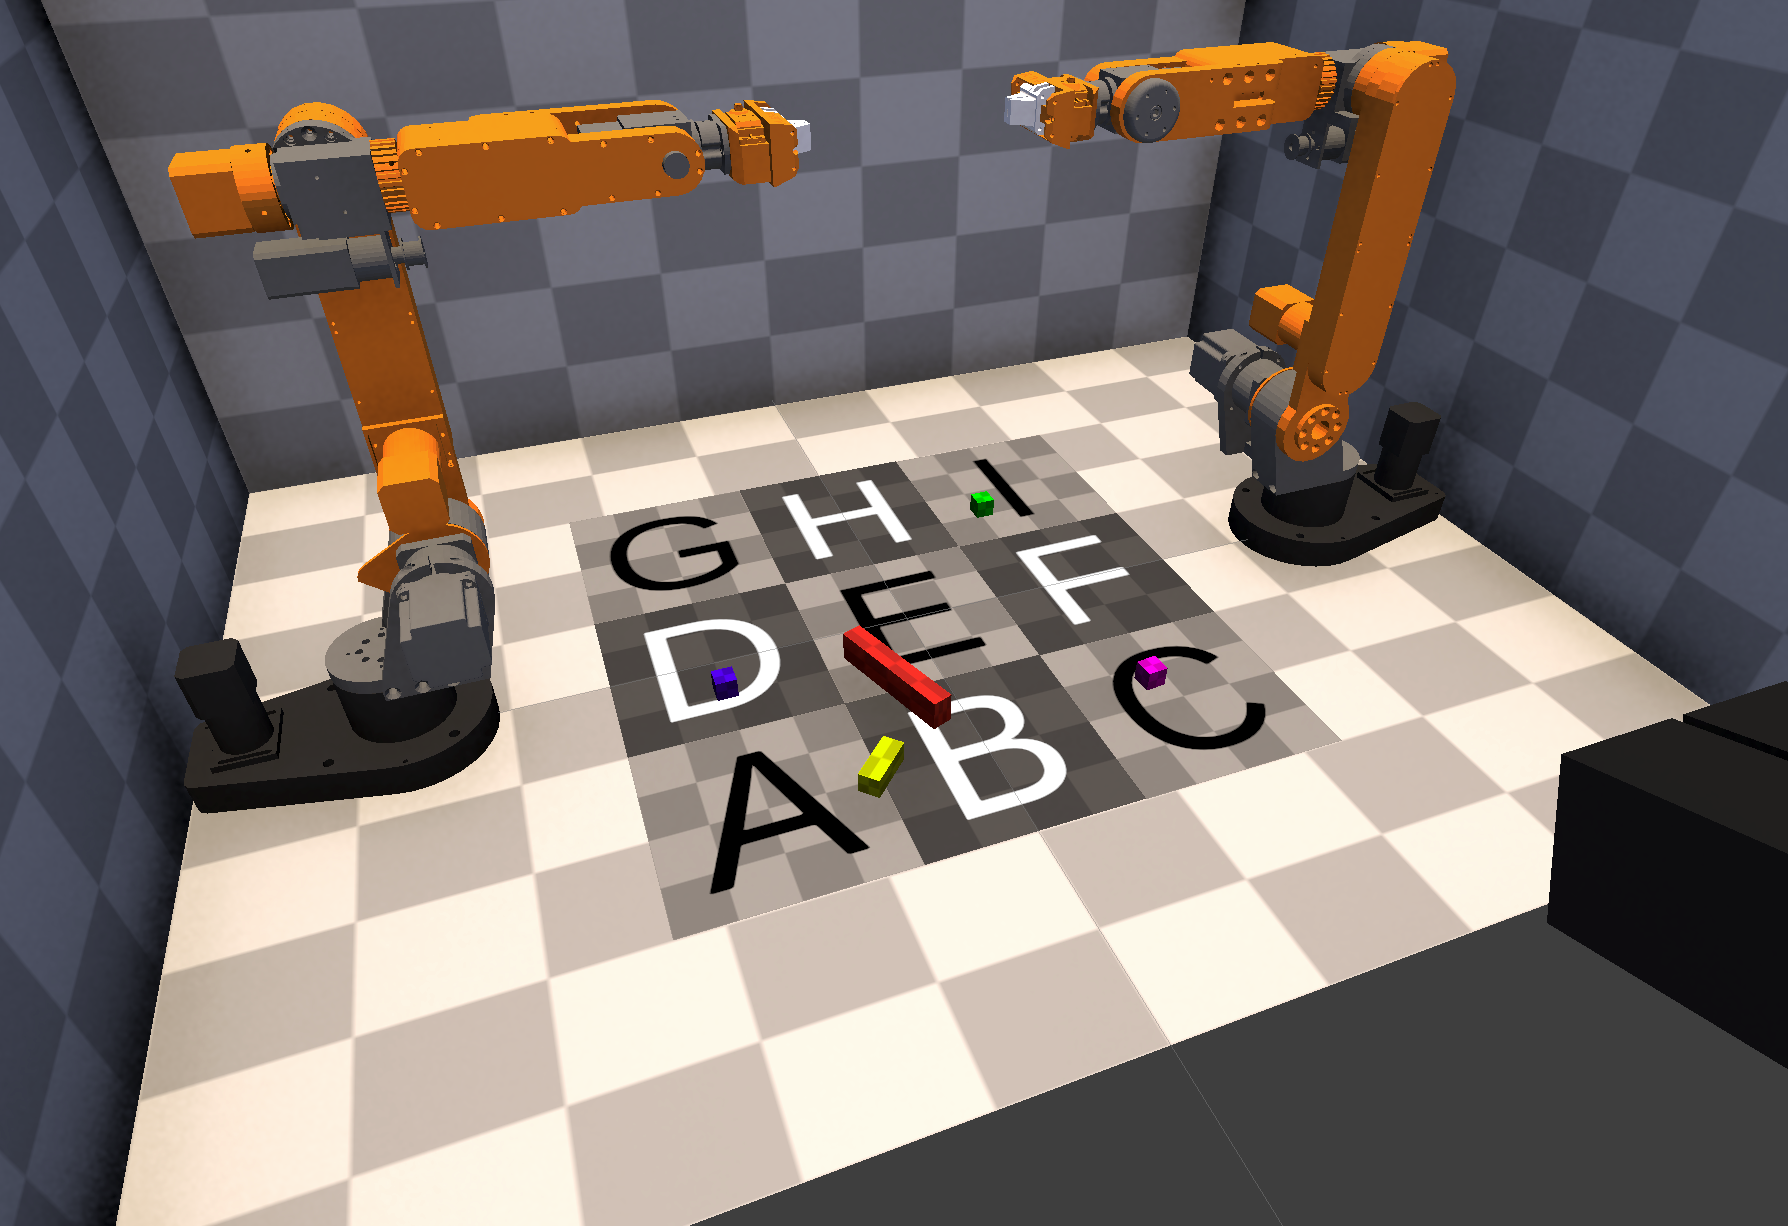
\includegraphics[width=\linewidth,height=0.5\textheight,keepaspectratio]{14_robot_env.png}\\
			\footnotesize Two AR4~\cite{AnninRobotics2026} arms, a shared workspace, and a stereo camera in Unity~\cite{unity}.
		\end{column}
	\end{columns}
\end{frame}

\begin{frame}{Two Design Commitments}
	\begin{columns}[t]
		\begin{column}{0.5\textwidth}
			\begin{block}{Run the model \emph{locally}}
				\begin{itemize}\small
					\item No cloud cost, no external dependency.
					\item No sensitive scene data leaving the machine.
					\item A compact VLM is enough; no frontier model required.
				\end{itemize}
			\end{block}
		\end{column}
		\begin{column}{0.5\textwidth}
			\begin{block}{Ground the model in \emph{modular operations}}
				\begin{itemize}\small
					\item Reasoning restricted to a vocabulary of \emph{executable} actions.
					\item Separates semantic understanding from physical execution, giving a predictable control rate.
					\item Vision resolves targets live; no task-specific training.
				\end{itemize}
			\end{block}
		\end{column}
	\end{columns}
	\vfill
	\centering\small Default backend model: \textbf{Magistral Small 2509 (24B, 4-bit)~\cite{mistral_magistral_small_2025}}
\end{frame}

\begin{frame}{Background}
	\begin{itemize}
		\item \textbf{End-to-end VLA} (RT-2, PaLM-E)~\cite{brohan2023rt2visionlanguageactionmodelstransfer,driess2023palmeembodiedmultimodallanguage}: great generalization, but data-hungry and opaque.
		\item \textbf{Code-as-Policies}~\cite{liang2023codepolicieslanguagemodel}: compositional and transparent, but tied to its API set.
		\item \textbf{Framework-scale} (ROS-LLM, AutoRT)~\cite{Mower_2026,ahn2024autortembodiedfoundationmodels}: practical scaffolding, but no joint reasoning over a \emph{shared} object.
		\item \textbf{RoCo}~\cite{mandi2023rocodialecticmultirobotcollaboration}: per-robot agents negotiate, but free-form way-points.
	\end{itemize}
	\vfill
	\begin{alertblock}{Research gap}
		Two arms reasoning \emph{jointly} about a single shared object, cooperation that \emph{emerges} from reasoning rather than being engineered from outside, is comparatively unexplored.
	\end{alertblock}
\end{frame}

% =============================================================================
% PILLAR 1 — GROUNDING -> RELIABILITY
% =============================================================================
\section{Pillar 1 --- Grounding}

\begin{frame}{System Architecture}
	\centering
	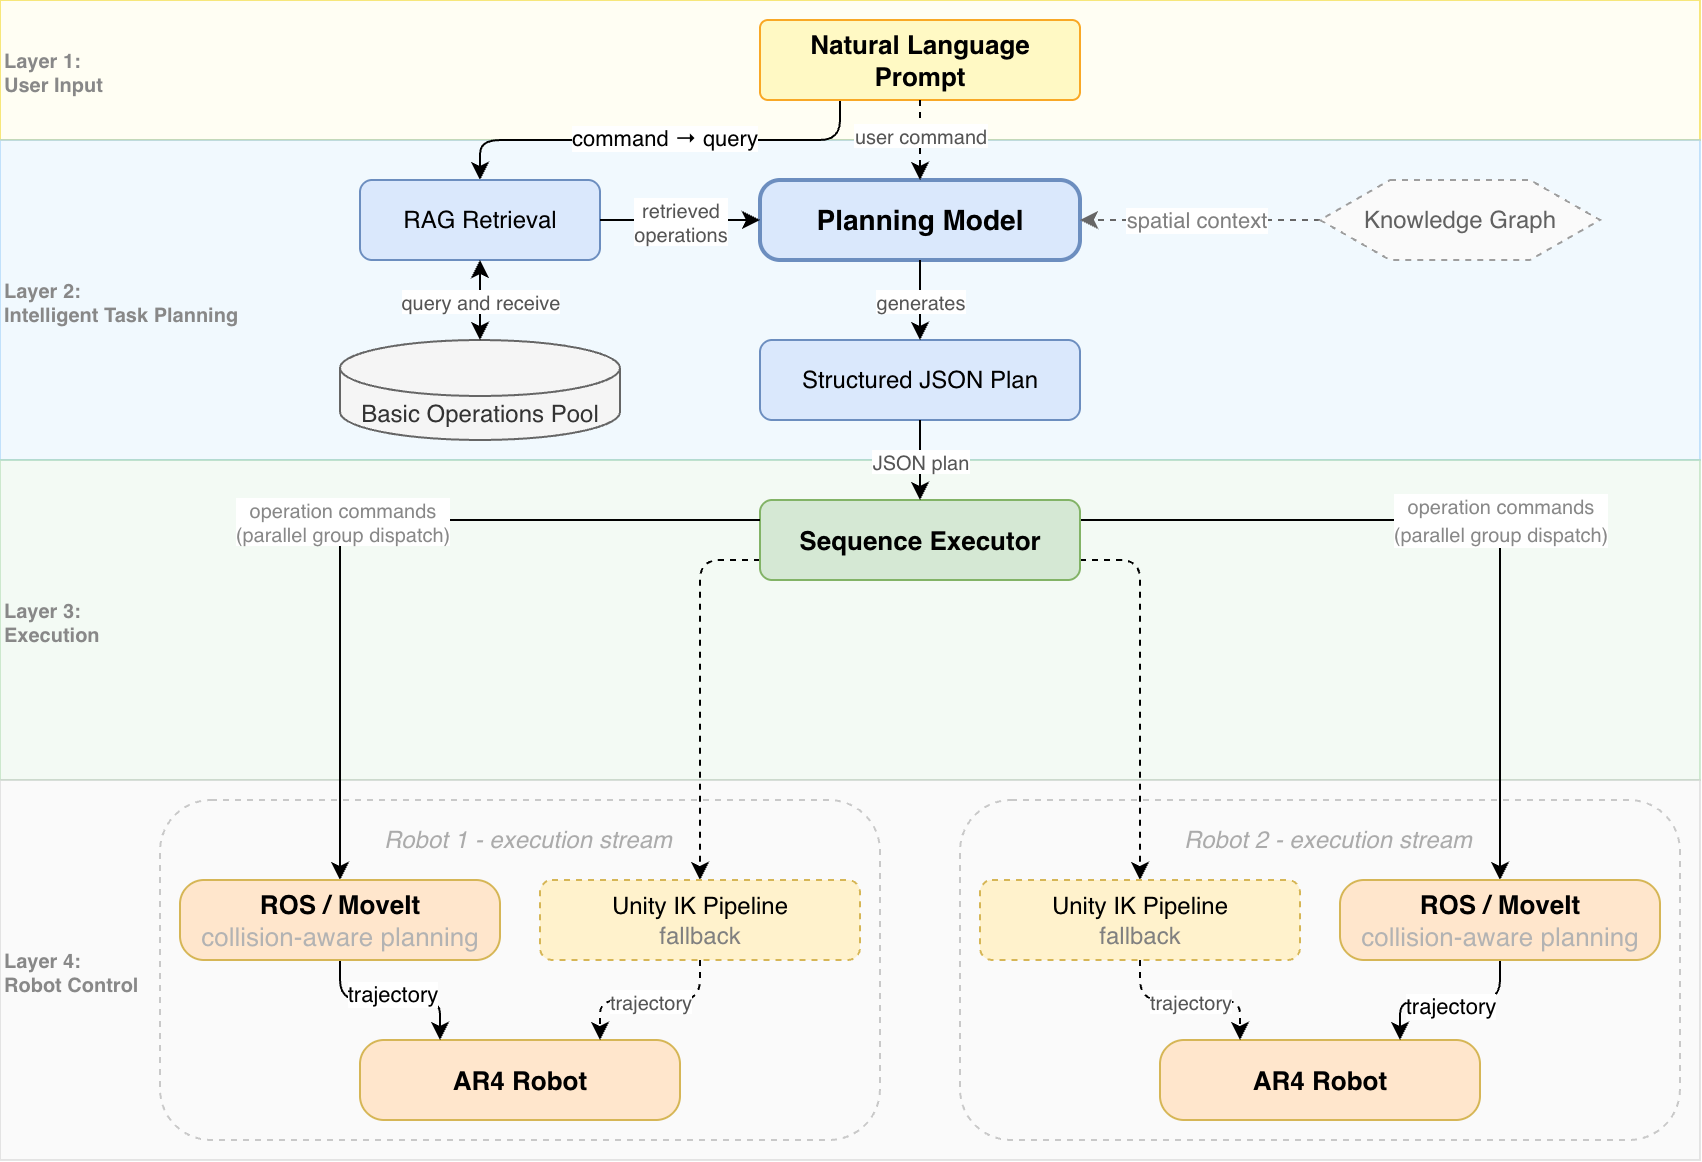
\includegraphics[height=0.75\textheight]{16_system_flow.png}\\
	\scriptsize Built on Unity, ROS~2~\cite{Macenski_2022}, and MoveIt~\cite{coleman2014reducingbarrierentrycomplex}.
\end{frame}

\begin{frame}{The Operation Pool}
	\begin{columns}[c]
		\begin{column}{0.5\textwidth}
			\footnotesize
			Operations organized by \textbf{complexity}, four tiers:
			\begin{description}\footnotesize
				\item[Atomic (8)] indivisible, no perception: gripper, signal, wait.
				\item[Basic (6)] single dispatch, introduces perception.
				\item[Intermediate (4)] composite single-robot: placement, stereo detection, scene analysis.
				\item[Complex (2)] full pipelines: grasp planning, handoff reception.
			\end{description}
			\vspace{0.3em}
			\textbf{Why it grounds:} model can only express plans the robot can actually run.
		\end{column}
		\begin{column}{0.5\textwidth}
			\centering
			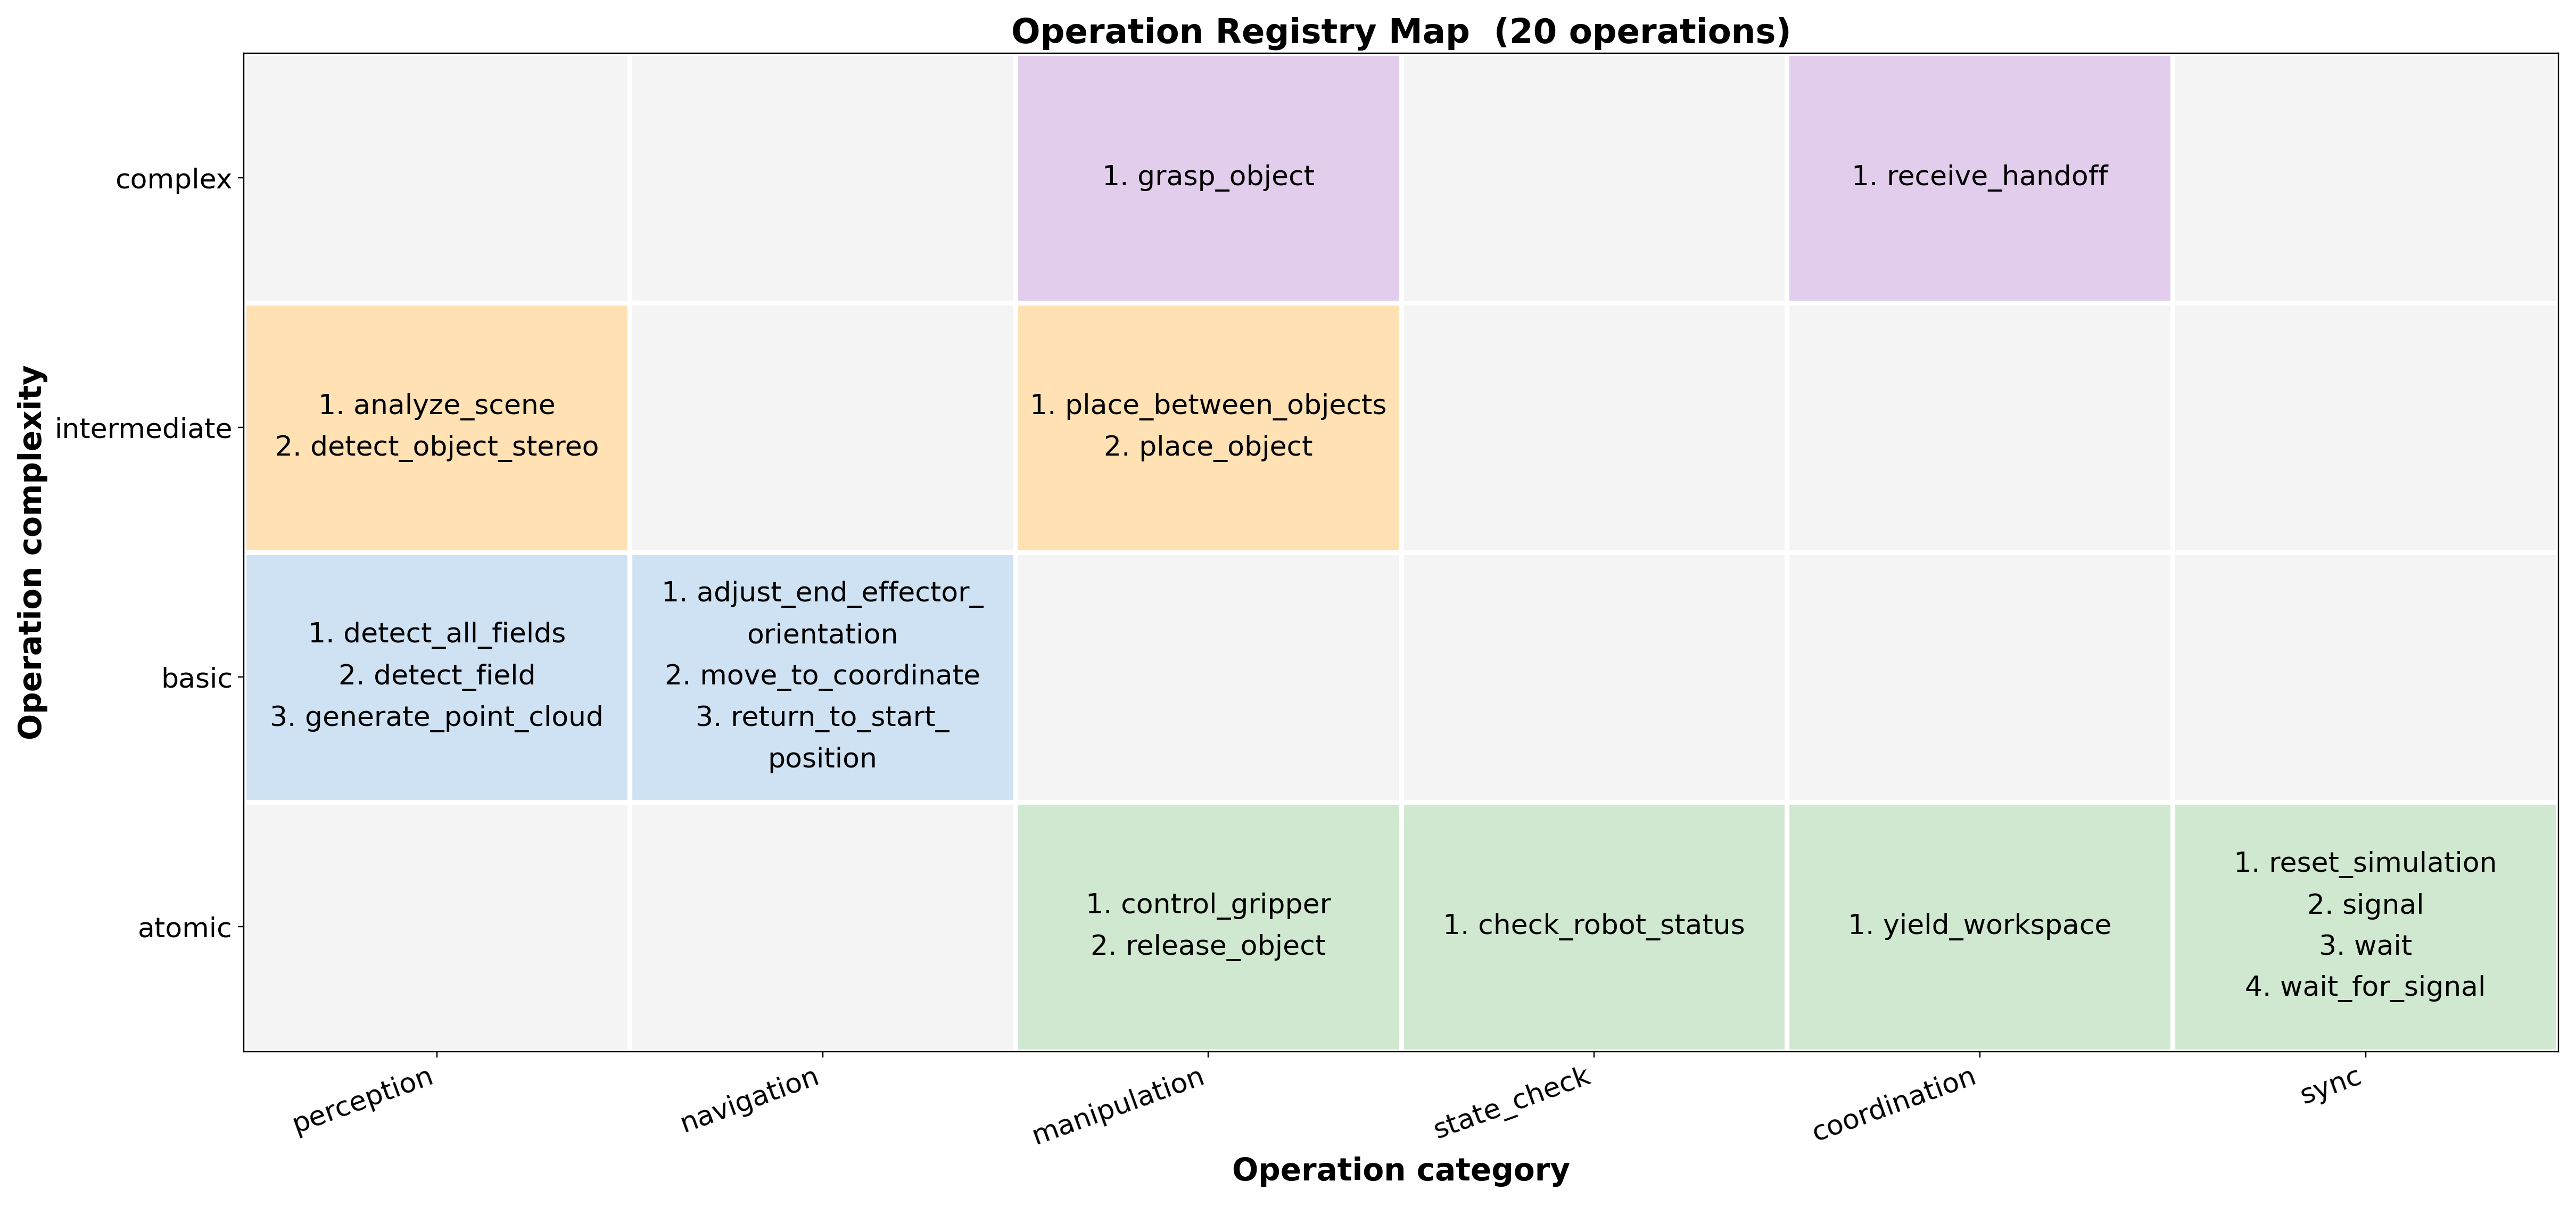
\includegraphics[width=\linewidth]{09_operation_map.png}
		\end{column}
	\end{columns}
\end{frame}

\begin{frame}{Two more Grounding Components}
	\begin{columns}[t]
		\begin{column}{0.5\textwidth}
			\begin{block}{Reflection recovery}
				\begin{itemize}\small
					\item On failure, re-query the model with a structured \emph{hint} and recovery suggestions (Reflexion-style verbal feedback~\cite{shinn2023reflexionlanguageagentsverbal}).
					\item Closes the perception--action loop at the language level.
					\item Eligibility is gated: no point re-querying a sync barrier.
				\end{itemize}
			\end{block}
		\end{column}
		\begin{column}{0.5\textwidth}
			\begin{block}{Knowledge graph}
				\begin{itemize}\small
					\item Robots / objects / regions as nodes; reachability, proximity, grasps as edges.
					\item Answers ``who can reach X?'', ``viable handoff?'' via multi-hop queries.
					\item \alert{Spoiler:} measured benefit is \emph{not} positive (Pillar 3).
				\end{itemize}
			\end{block}
		\end{column}
	\end{columns}
\end{frame}

\begin{frame}{Grounding $\Rightarrow$ Reliability}
	\begin{columns}[c]
		\begin{column}{0.5\textwidth}
			\begin{itemize}\small
				\item \textbf{B1--B5} (navigate $\to$ grasp $\to$ full pick-and-place): \alert{success over all 25 runs}, zero hallucinated ops, zero retries.
				\item \emph{Identical} operation sequence on all 5 runs of each benchmark.
				\item \textbf{B8} (long chain): 20 sub-tasks, \textbf{85 operations}/run, 5 cycles, all executed, no cascading errors.
			\end{itemize}
			\vspace{0.4em}
			\footnotesize Cost is dominated by \emph{contact-rich} primitives (\texttt{grasp\_object}, \texttt{place\_object}).
		\end{column}
		\begin{column}{0.5\textwidth}
			\centering
			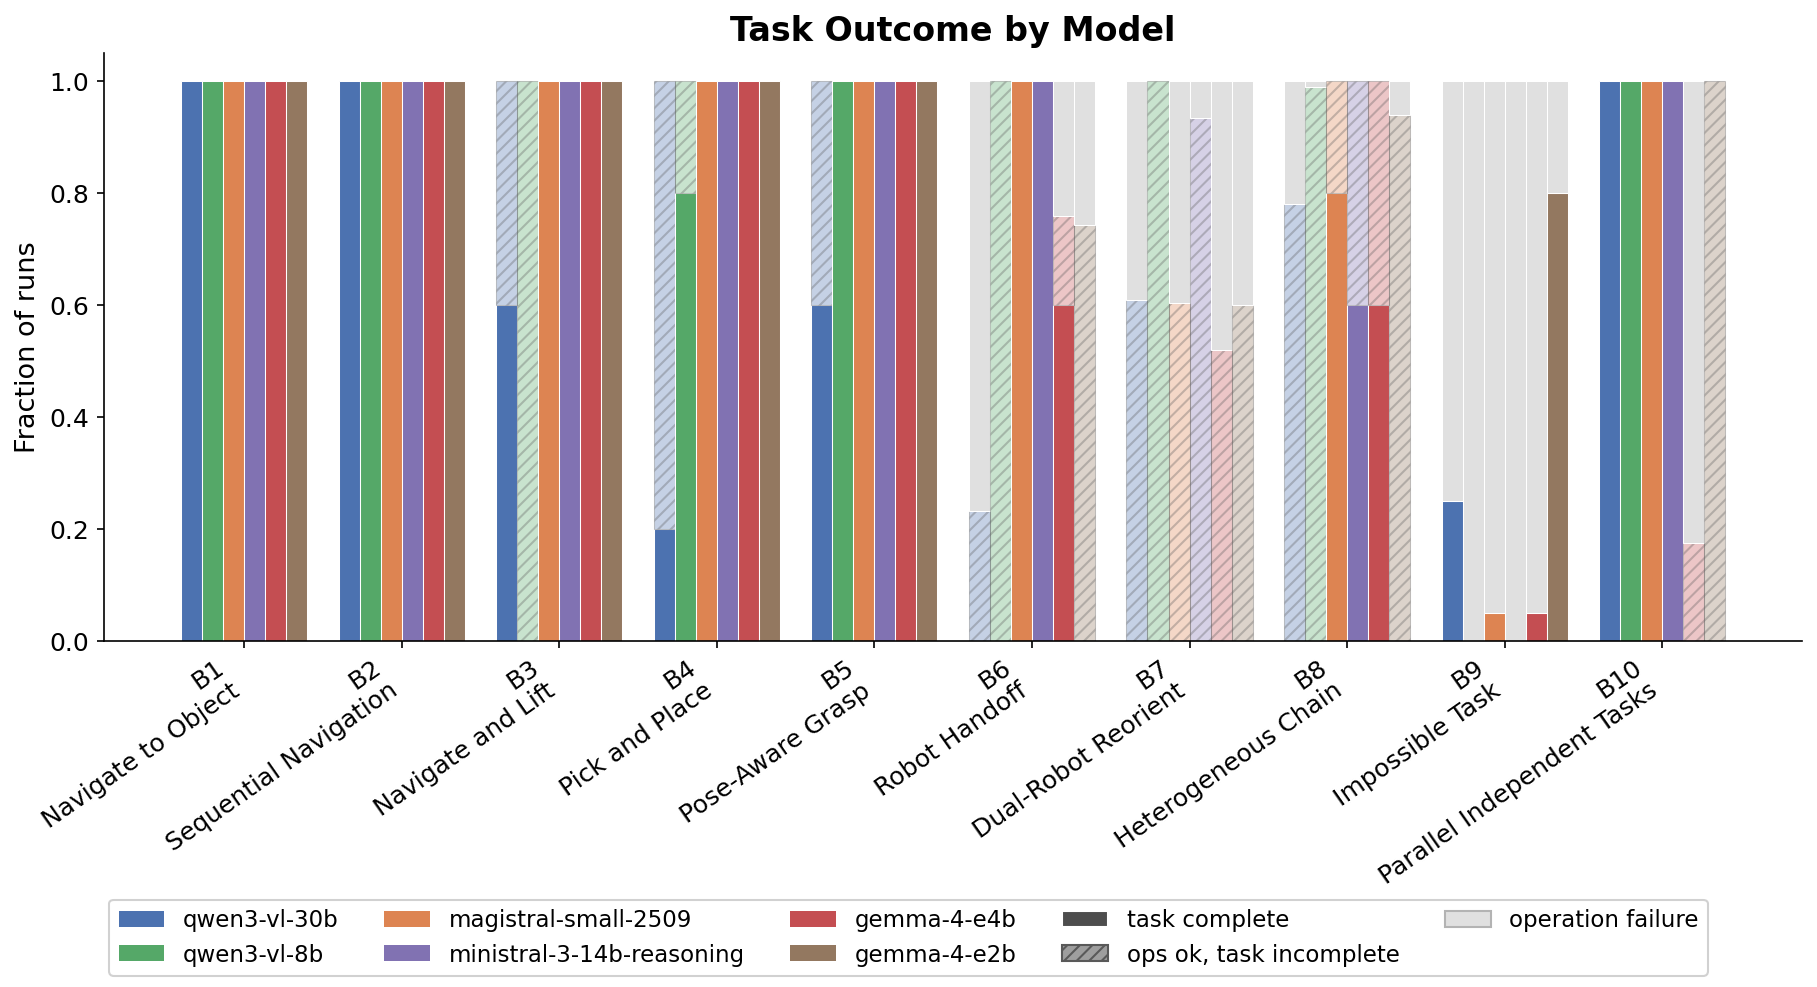
\includegraphics[width=\linewidth]{01_success_rate_by_model.png}\\
			\footnotesize Magistral, Ministral, and both Gemma~4 models clear the full single-robot gradient; the Qwen3-VL models fail from B3 onward by truncating plans.
		\end{column}
	\end{columns}
\end{frame}

% =============================================================================
% PILLAR 2 — COOPERATION EMERGES
% =============================================================================
\section{Pillar 2 --- Cooperation Emerges}

\begin{frame}{The Model Composes}
	\begin{block}{Two general primitives}
		\begin{itemize}
			\item \texttt{signal} / \texttt{wait\_for\_signal}: one robot pauses at a checkpoint until the other signals readiness.
			\item \textbf{Parallel groups}: operations dispatched concurrently when no ordering is needed.
		\end{itemize}
	\end{block}
	\vfill
	The executor imposes \alert{no} coordination policy. The model decides \emph{where} synchronization is needed and \emph{which} steps can run in parallel, guided only by general rules in the prompt, never an explicit script.
\end{frame}

\begin{frame}{The Handoff}
	\begin{columns}[c]
		\begin{column}{0.5\textwidth}
			\begin{itemize}
				\item Magistral and Ministral: 5/5 runs; all operations succeed first try.
				\item The plan places a \textbf{synchronization barrier} so Robot2 receives only after Robot1 signals.
				\item Gemma-4B partial (3/5); the Qwen3 models and Gemma-2B break down at plan construction.
			\end{itemize}
		\end{column}
		\begin{column}{0.5\textwidth}
			\centering
			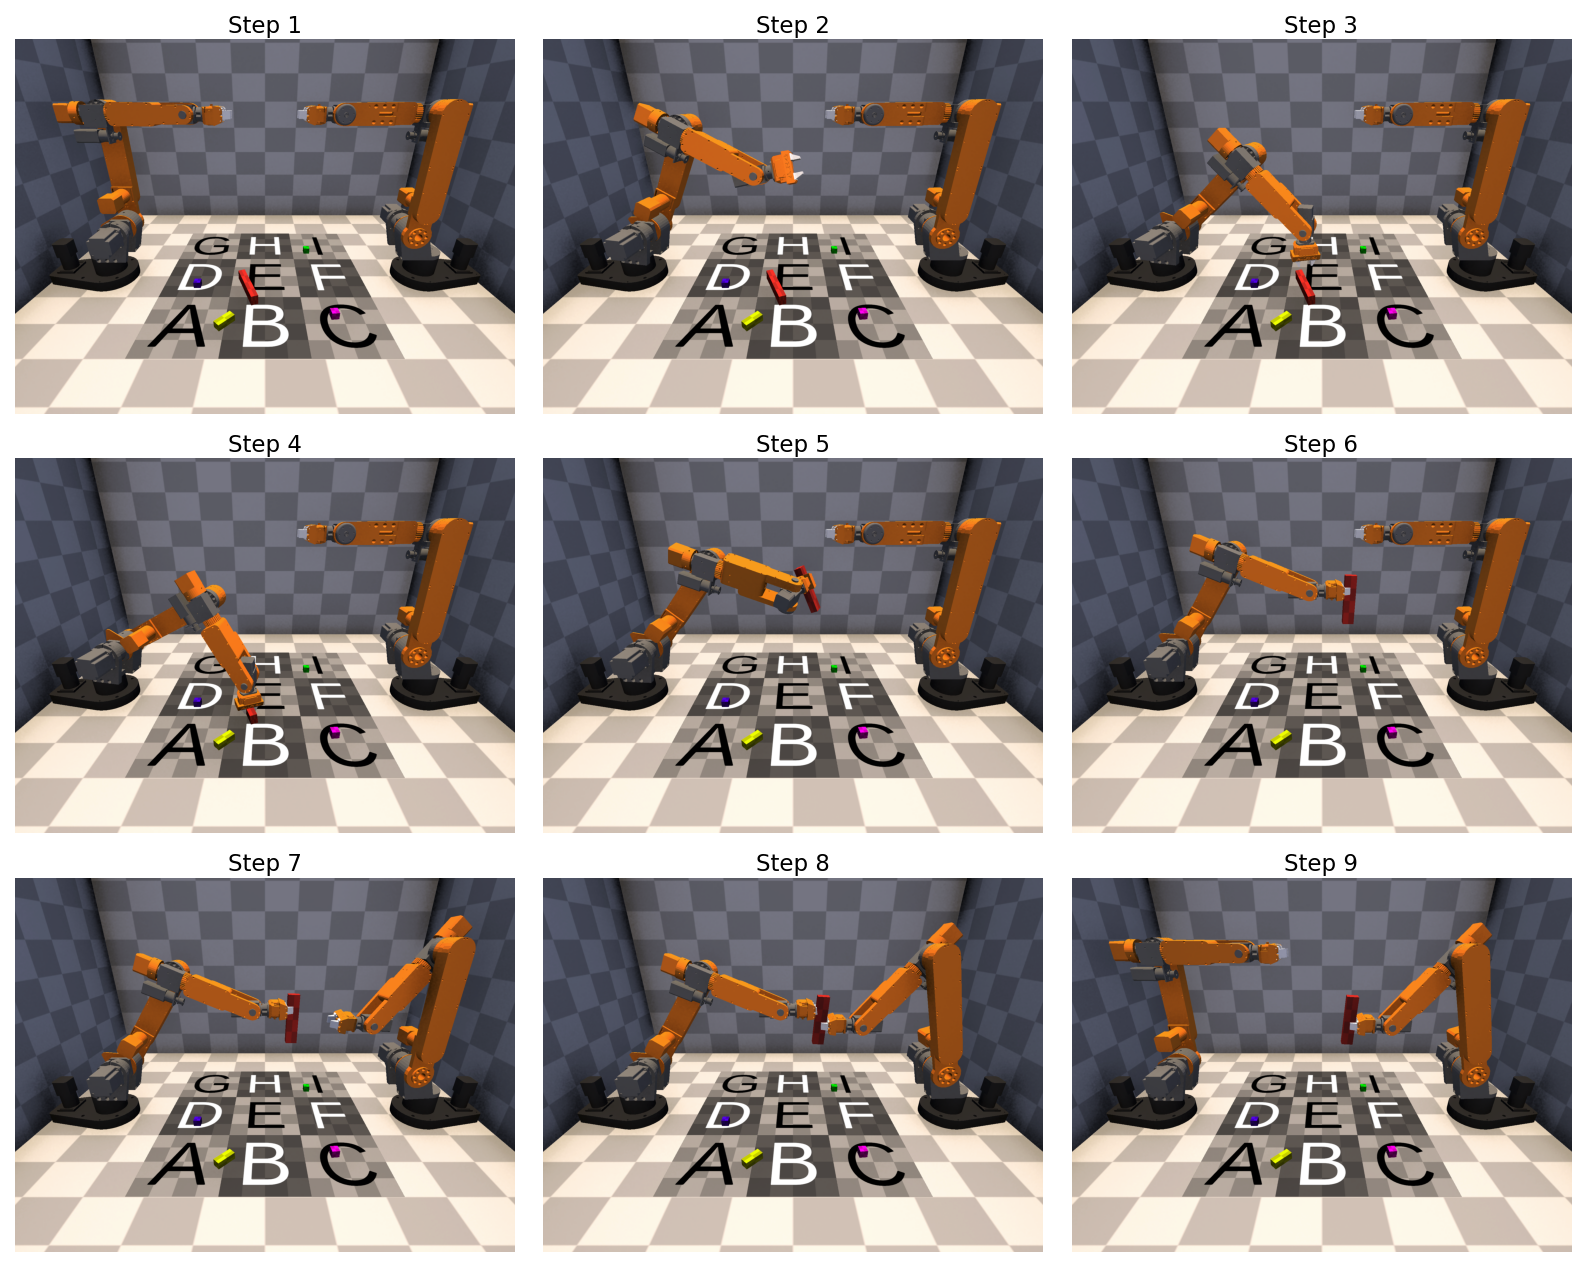
\includegraphics[width=\linewidth]{18_handoff_sequence_example.png}\\
			\footnotesize Handoff sequence.
		\end{column}
	\end{columns}
\end{frame}

\begin{frame}{Emergent Parallelism}
	\begin{itemize}
		\item 4/6 models: 40/40 operations, zero retries.
		\item Applying the prompt's independent-parallel rule.
		\item Heavy manipulation phases run concurrently; detection kept sequential, a conservative, stable choice.
	\end{itemize}
	\vfill
	\begin{exampleblock}{Takeaway}
		The model expresses physical simultaneity when the task allows it, the same capability that matters for the unsolved B7.
	\end{exampleblock}
\end{frame}

\begin{frame}{Negotiation}
	\begin{columns}[T]
		\begin{column}{0.55\textwidth}
			\footnotesize
			A single model planning both arms under-specifies roles; \emph{implicit conflicts} surface only at execution.
			\vfill
			\textbf{Protocol}:
			\begin{enumerate}\setlength{\itemsep}{0pt}
				\item \textbf{Analyze}: each agent assesses its own role (parallel).
				\item \textbf{Propose}: one agent/round drafts a \emph{complete} plan (round-robin).
				\item \textbf{Evaluate}: peers accept/reject with justification; \alert{unanimity} required. Rejections feed the next proposal.
			\end{enumerate}
			No consensus in 3 rounds $\to$ single-model parsing.
		\end{column}
		\begin{column}{0.48\textwidth}
			\centering
			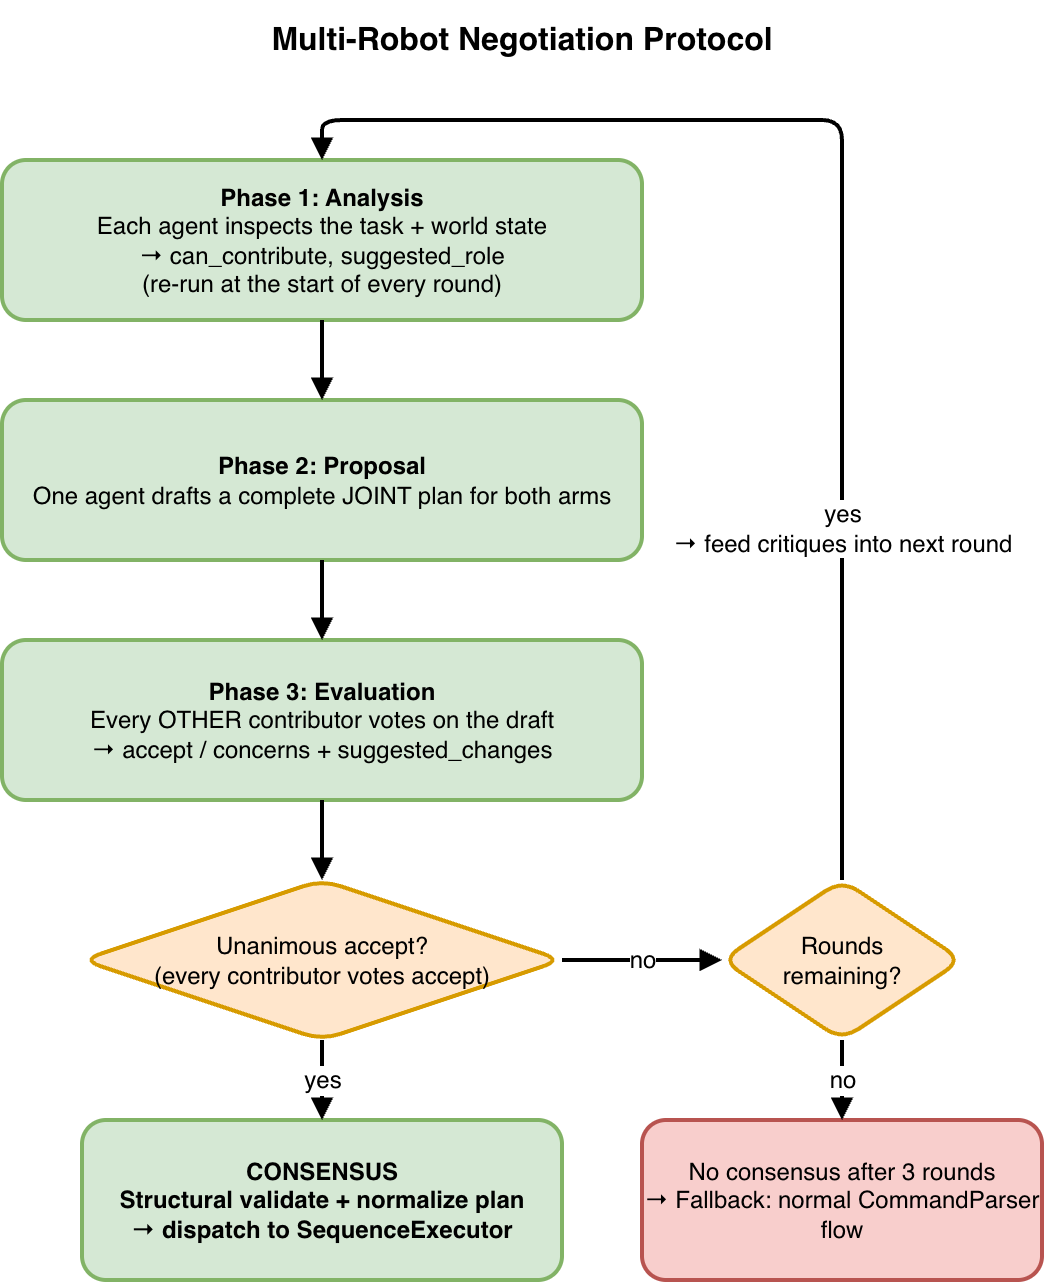
\includegraphics[height=0.8\textheight]{19_negotiation.png}
		\end{column}
	\end{columns}
\end{frame}

\begin{frame}{Negotiation Pays Off}
	\begin{columns}[c]
		\begin{column}{0.5\textwidth}
			\begin{table}\footnotesize
				\begin{tabular}{lcc}
					\toprule
					                        & \textbf{Task SR}      & \textbf{Ops/run} \\
					\midrule
					Negotiation \textbf{on} & \alert{0.713} (57/80) & 35.8             \\
					Negotiation off         & 0.613 (49/80)         & 29.9             \\
					\bottomrule
				\end{tabular}
			\end{table}
			\vspace{0.4em}
			\footnotesize
			\begin{itemize}
				\item \alert{+10 pp} task success for the \textbf{default model}.
				\item Roughly neutral for three backends; \emph{negative} for two ($-19$, $-21$ pp).
				\item Pays off when the single-shot plan is already close to correct; doesn't rescue weaker planners from role conflicts.
			\end{itemize}
		\end{column}
		\begin{column}{0.5\textwidth}
			\centering
			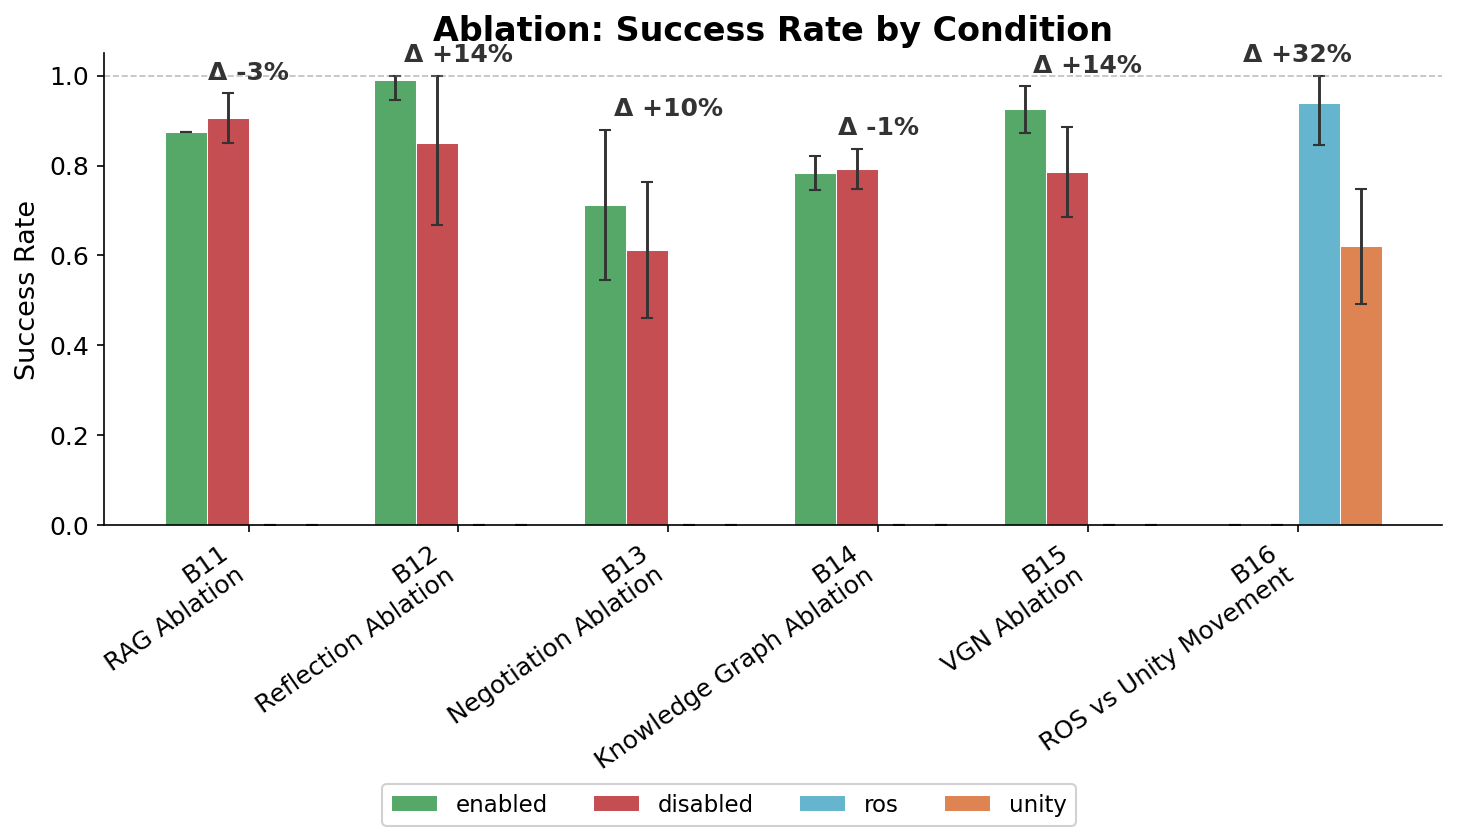
\includegraphics[width=\linewidth]{08_ablation.png}\\
			\footnotesize Per-component ablation deltas (Magistral; $n=20$ for B11--B13, B16; $n=5$ for B14--B15).
		\end{column}
	\end{columns}
\end{frame}

% =============================================================================
% PILLAR 3 — THE BOUNDARY  (~6 min)
% =============================================================================
\section{Pillar 3 --- The Boundary}

\begin{frame}{Concurrent Bimanual Lift}
	\begin{columns}[T]
		\begin{column}{0.5\textwidth}
			\textbf{All six models fail.} Three failure modes:
			\begin{enumerate}\footnotesize
				\item Signal primitives never dispatched once control crosses robots outside a parallel group.
				\item Final lift: two \emph{independently} chosen targets land too close together, violating the separation check.
				\item Deeper sim limit: a Unity \texttt{Transform} has one parent, so a single object can't attach to two grippers at once.
			\end{enumerate}
		\end{column}
		\begin{column}{0.5\textwidth}
			\begin{block}{The gap}
				\footnotesize
				\alert{Partner-aware target selection}. Each arm picks a valid target; nothing checks one \emph{against the other}.
			\end{block}
		\end{column}
	\end{columns}
\end{frame}

\begin{frame}{Ablation Synthesis}
	\begin{table}\scriptsize
		\begin{tabular}{lll}
			\toprule
			\textbf{Component}                                                    & \textbf{Effect}   & \textbf{Reading}                                                     \\
			\midrule
			ROS/MoveIt                                                            & +32 pp            & Unity-only grasp timeouts; plus collision-aware planning             \\
			Reflection                                                            & +14 pp (task)     & Clears boundary-reach failures; +7 pp op; doubles time when it fires \\
			Negotiation                                                           & +10 pp            & Default model only; neutral/negative on the other five               \\
			RAG~\cite{lewis2021retrievalaugmentedgenerationknowledgeintensivenlp} & net cost          & Helps no backend; \alert{hurts} 3 of 6 ($-7$ pp pooled)              \\
			Knowledge graph                                                       & small \emph{cost} & Prompt over-anchoring, not a broken component                        \\
			VGN grasp                                                             & +35 pp Magi       & center-of-object grasp, not predicted orientation                    \\
			                                                                      & (+33 pp pooled)   &                                                                      \\
			\bottomrule
		\end{tabular}
	\end{table}
	\vfill
	\begin{block}{Caveat}
		\scriptsize Point estimates, one simulated environment: \textbf{$n=20$} per condition for RAG, Reflection, Negotiation and ROS, $n=5$ for the knowledge graph and ROS. Enough to expose deterministic failure modes, not to resolve effects within one standard deviation.
	\end{block}
\end{frame}

\begin{frame}{AutoRT Adaptation \& Safety Gate}
\begin{columns}[c]
\begin{column}{0.5\textwidth}
	Re-targeted AutoRT for \emph{fixed-base} manipulation.
	\vspace{0.4em}

	\textbf{Two-layer safety (Robot Constitution):}
	\begin{itemize}
		\item Semantic VLM check
		\item Hard kinematic check the semantic layer can't override.
	\end{itemize}
	\vspace{0.3em}
	Result: never admits an unsafe task. Slightly over-rejects aggressive-but-safe phrasing.
\end{column}
\begin{column}{0.5\textwidth}
	\centering
	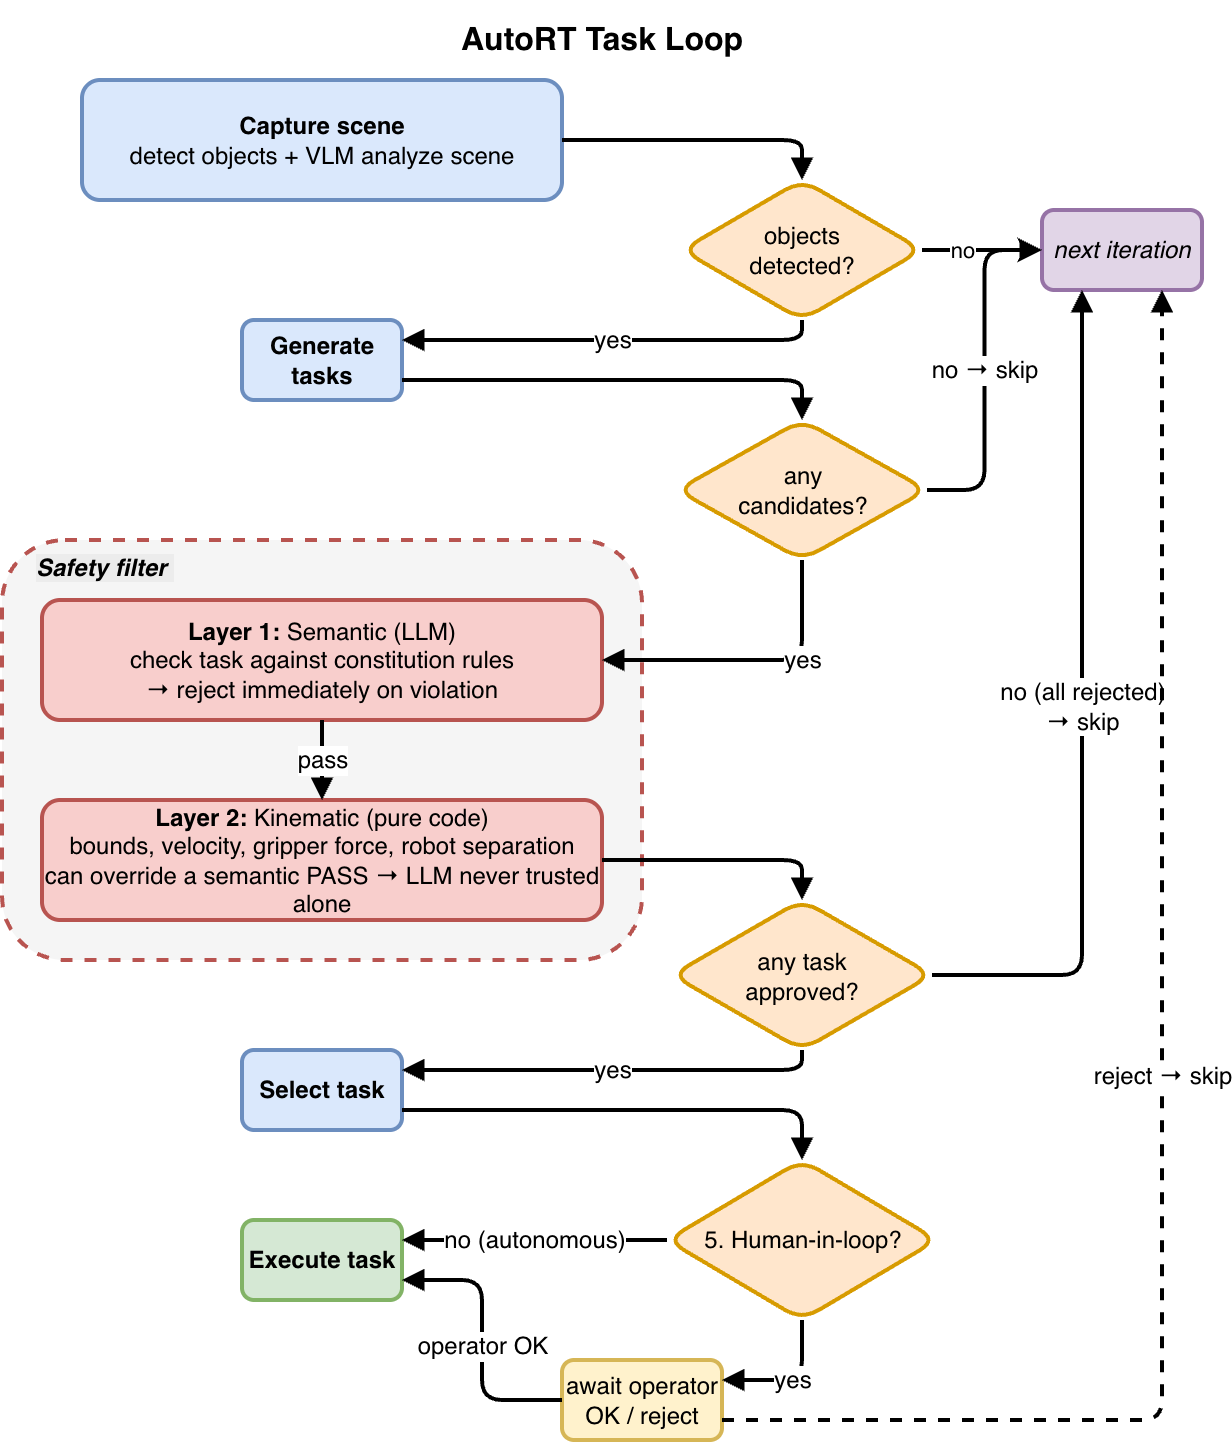
\includegraphics[height=0.85\textheight]{20_autort.png}
\end{column}
\end{columns}
\end{frame}

\begin{frame}{Limitations}
	\begin{columns}[t]
		\begin{column}{0.5\textwidth}
			\begin{block}{Sensing}
				\footnotesize Stereo depth degrades on textureless surfaces, so VGN's predicted poses are overridden by the top-down heuristic.
			\end{block}
			\begin{block}{Latency}
				\footnotesize VLM parse $\approx$ \textbf{20\,s} median, which prevents \emph{reactive} control; re-plan only between motions, never during.
			\end{block}
		\end{column}
		\begin{column}{0.5\textwidth}
			\begin{block}{Sim-to-real}
				\footnotesize Robot joint values all tuned for simulation, so they need revalidation on hardware.
			\end{block}
			\begin{block}{Validation}
				\footnotesize 5/6 models forward impossible inputs; the guard must be pre-parse.
			\end{block}
		\end{column}
	\end{columns}
\end{frame}

% =============================================================================
% CLOSE
% =============================================================================
\section{Conclusion}

\begin{frame}{Five Contributions}
	\begin{enumerate}\small
		\item \textbf{Retrieval-grounded operation pipeline}: a hierarchical 20-operation registry retrieved on demand via RAG, with two-phase decomposition and runtime variable-passing. No hard-coded sequences, no fine-tuning.
		\item \textbf{Runtime-composed coordination}: handoff, parallelism, and waiting built from general \texttt{signal}/\texttt{wait} and parallel-group primitives, not scripted into the executor.
		\item \textbf{Consensus-gated negotiation}: per-robot agents analyze/propose/evaluate under unanimity; +10~pp on role-ambiguous tasks for the default model.
		\item \textbf{Operation-gated reflection}: retry with functional recovery hints on eligible failures; +14~pp task success for the default model.
		\item \textbf{AutoRT adaptation}: fixed-base task generation plus a two-layer Robot Constitution with a hard kinematic layer the semantic check cannot override.
	\end{enumerate}
\end{frame}

\begin{frame}{Path to a Real Robot}
	\begin{itemize}
		\item Hardware abstraction boundary: \texttt{--env real} swaps camera and hardware adapters.
		\item Switch control to \textbf{ROS}: ROS/MoveIt collision-aware planning, the correct route for physical AR4 hardware, already dual-robot configured.
	\end{itemize}
	\vfill
	\begin{block}{Two remaining blockers}
		\footnotesize
		\textbf{Depth sensing}: a LIDAR source unlocks the VGN pipeline.\\
		\textbf{Force-torque feedback}: a wrist sensor replaces the contact-duration heuristic.
	\end{block}
\end{frame}

\begin{frame}{Future Work}
	\begin{itemize}
		\item \textbf{Depth upgrade}: a LIDAR sensor fully unlocks VGN-grade grasping.
		\item \textbf{Persistency}: a persistent volumetric map using SLAM
		\item \textbf{Bimanual pre-pass}: detect simultaneous grasp language, route to a bimanual-aware prompt to solve bimanual gap.
		\item \textbf{Pre-parse validation}: robot-ID and object-existence checks before any model call.
		\item \textbf{Faster inference}: distilled task-specific models and/or speculative parsing to shrink the 20\,s window.
	\end{itemize}
\end{frame}

\section*{Summary}

\begin{frame}{Summary}
	\begin{columns}[T]
		\begin{column}{0.5\textwidth}
			\footnotesize
			\textbf{What works}
			\begin{itemize}\scriptsize
				\item Single-robot: works in 25/25 runs.
				\item Long chain: 85 ops/run, 5 cycles, no cascading errors.
				\item Handoff: works and correctly realized sync barrier.
				\item Parallelism: works for 4/6 backends.
				\item Safety gate: no false-accept, reproducible.
			\end{itemize}

		\end{column}
		\begin{column}{0.5\textwidth}
			\footnotesize
			\textbf{What each component contributes}
			\begin{itemize}\scriptsize
				\item VGN grasp: +35 pp Magistral, +33 pp pooled.
				\item ROS/MoveIt: +32 pp, Unity-only grasp timeouts.
				\item Reflection: +14 pp task.
				\item Negotiation: +10 pp, default model only.
				\item RAG: model-dependent; KG (B14): small cost.
			\end{itemize}
			\vspace{0.3em}
			\textbf{The one open gap}
			\begin{itemize}\scriptsize
				\item Concurrent bimanual B7: all six models fail.
				\item Cause: partner-aware target selection.
			\end{itemize}
		\end{column}
	\end{columns}
\end{frame}

% =============================================================================
% END
% =============================================================================

\begin{frame}[standout]
	\centering
	Demo \& Questions
	\vfill
	\footnotesize \texttt{github.com/JanMStraub/Cooperative-Robot-Behavior-from-Basic-Action-Modules}
\end{frame}

\begin{frame}[t]{References}
	\begin{multicols}{2}
		\bibliographystyle{IEEEtran}
		\bibliography{references}
	\end{multicols}
\end{frame}

% =============================================================================
% BACKUP
% =============================================================================
\appendix
\setbeamertemplate{frame numbering}{}  % no page numbers on backup/reference slides

\section*{Additional Slides}

\begin{frame}[noframenumbering]{Backup ---  Bimanual Lift per-run Outcomes}
	\begin{table}\footnotesize
		\begin{tabular}{ccll}
			\toprule
			\textbf{Run} & \textbf{Ops ok} & \textbf{Dur (s)} & \textbf{Failing op}                       \\
			\midrule
			1            & 4/8             & 111              & \texttt{wait\_for\_signal}                \\
			2            & 4/10            & 43               & \texttt{wait\_for\_signal}                \\
			3            & 6/7             & 211              & \texttt{move\_to\_coordinate} (collision) \\
			4            & 6/7             & 206              & \texttt{move\_to\_coordinate} (collision) \\
			5            & 4/10            & 46               & \texttt{wait\_for\_signal}                \\
			\bottomrule
		\end{tabular}
	\end{table}
	\footnotesize Two clusters: mis-realized barrier, never executed (1,2,5), and lift-target collision at $\sim$0.10\,m (3,4).
\end{frame}

\begin{frame}[noframenumbering]{Backup --- What VGN~\cite{breyer2021volumetricgraspingnetworkrealtime} changes}
	\begin{columns}[T]
		\begin{column}{0.47\textwidth}
			\begin{table}\scriptsize
				\begin{tabular}{lcc}
					\toprule
					\textbf{Held \& lifted} & \textbf{VGN on}       & \textbf{VGN off} \\
					\midrule
					Magistral               & \alert{14/20 (0.700)} & 7/20 (0.350)     \\
					Pooled, 6 models        & \alert{0.750}         & 0.417            \\
					\bottomrule
				\end{tabular}
			\end{table}
			\footnotesize
			\begin{itemize}\footnotesize
				\item Every backend improves: +20\,pp (Ministral) to +65\,pp (Gemma-4B).
				\item Success = held and lifted clear of the table.
			\end{itemize}
		\end{column}
		\begin{column}{0.53\textwidth}
			\begin{block}{Mechanism: position, not orientation}
				\footnotesize
				\begin{itemize}\footnotesize
					\item \textbf{Same orientation both conditions}: top-down, yaw from the object's long axis. VGN's own poses fail motion planning and are discarded.
					\item \textbf{The difference is position}: VGN grasps the detected object \emph{center}; the baseline's contact point sits off-center on angled cubes and slips.
				\end{itemize}
			\end{block}
			\begin{block}{Scope}
				\footnotesize Position comes from the WorldState oracle, so B15 isolates grasp \emph{positioning}. Recovering VGN's learned pose needs a real depth sensor.
			\end{block}
		\end{column}
	\end{columns}
\end{frame}

\begin{frame}[noframenumbering]{Backup --- Collision Safety Layers}
	\begin{columns}[T]
		\begin{column}{0.52\textwidth}
			\footnotesize
			\begin{enumerate}\footnotesize
				\item \textbf{Static pre-check} (Python, before dispatch): \texttt{CoordinationVerifier} checks workspace bounds, object conflicts, deadlock detection on the planned targets.
				\item \textbf{Workspace regions}: left / right / shared zones; a contested zone is handed over explicitly via \texttt{yield\_workspace}.
				\item \textbf{Runtime guard} (Unity, every physics step): \texttt{ProximityGuard} freezes motion at 0.25\,m end-effector distance, resumes at 0.35\,m; link-to-link limit 0.15\,m.
			\end{enumerate}
			\vspace{0.4em}
			The LLM is never trusted for safety: layers 1 and 3 are code, not reasoning.
		\end{column}
		\begin{column}{0.48\textwidth}
			\centering
			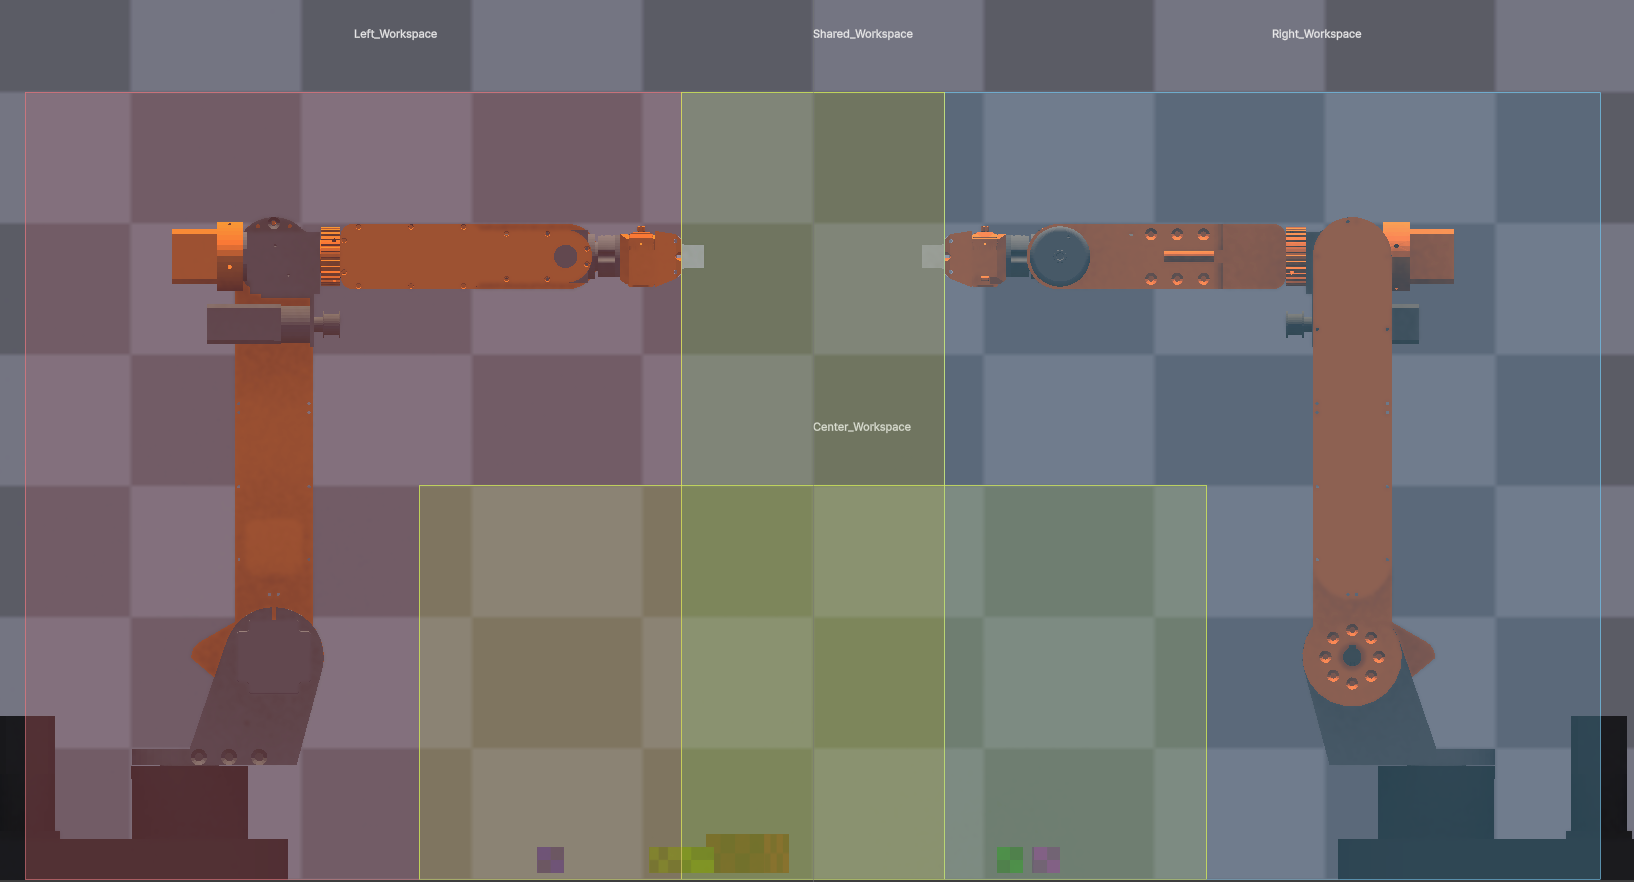
\includegraphics[width=\linewidth]{15_robot_workspaces.png}
		\end{column}
	\end{columns}
\end{frame}

\begin{frame}[noframenumbering]{Backup --- Single-Robot Operation Latencies}
	\begin{table}\footnotesize
		\begin{tabular}{llcc}
			\toprule
			\textbf{Operation}              & \textbf{Bench} & \textbf{n} & \textbf{Mean (s)} \\
			\midrule
			\texttt{detect\_object\_stereo} & B1--B5         & 30         & 0.80              \\
			\texttt{move\_to\_coordinate}   & B1--B3         & 20         & 4.37              \\
			\texttt{grasp\_object} (B3)     & B3             & 5          & 19.84             \\
			\texttt{grasp\_object} (B4)     & B4             & 5          & 10.93             \\
			\texttt{place\_object}          & B4             & 5          & 34.43             \\
			\bottomrule
		\end{tabular}
	\end{table}
	\footnotesize Perception is cheap and stable; contact-rich manipulation dominates and varies with object pose.
\end{frame}

\begin{frame}[noframenumbering]{Backup --- Model $\times$ Task Matrix}
	\centering
	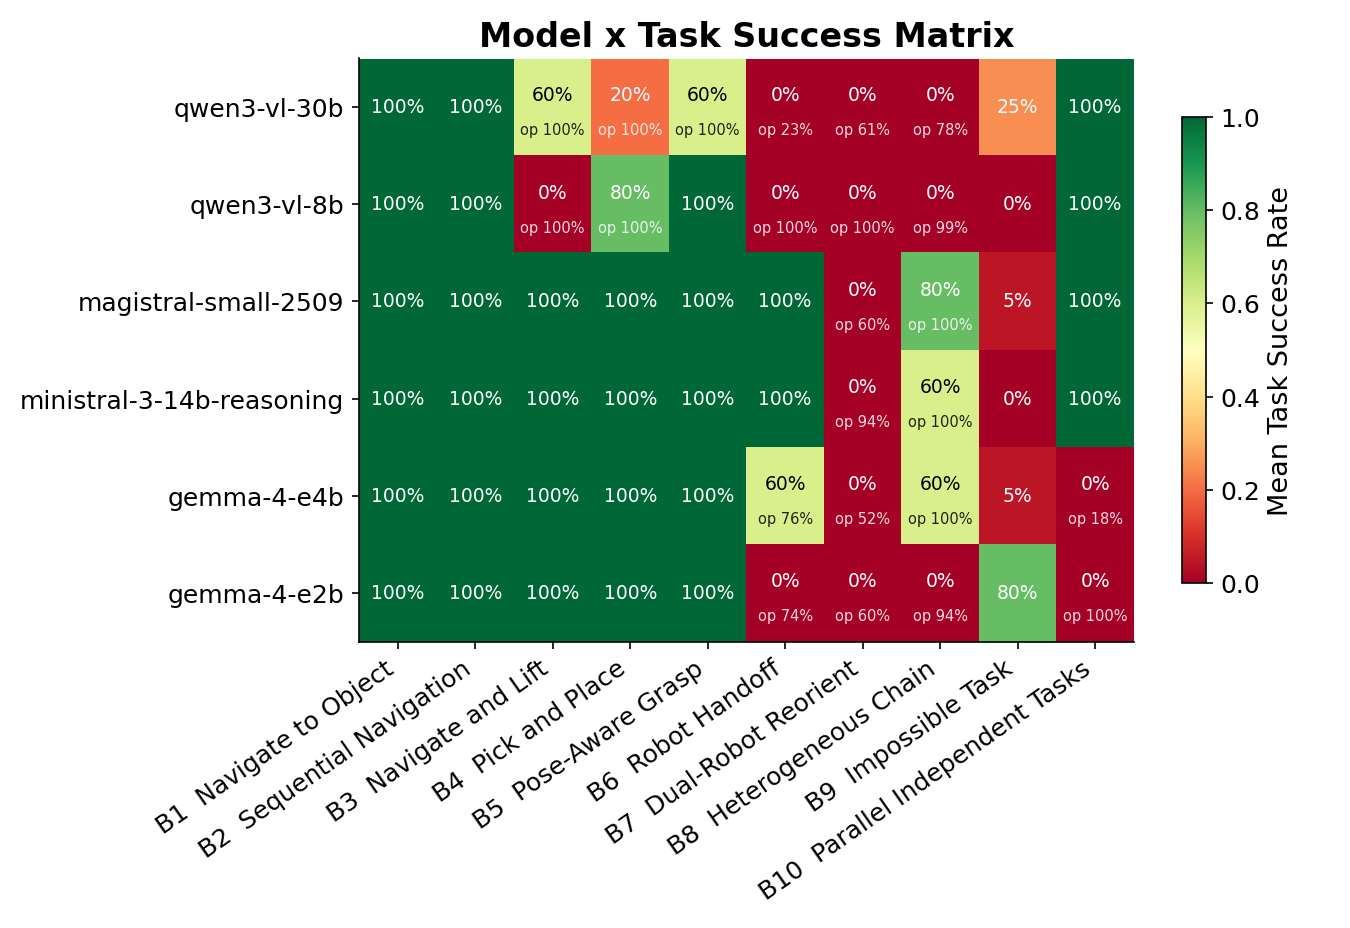
\includegraphics[height=0.8\textheight]{02_model_task_heatmap.png}
\end{frame}

\end{document}
